\chapter{Literature}
\label{chapter:Literature}

Cellular automata (CA) models have been widely used to simulate traffic flow. This section presents the key papers that form the basis of this thesis.

\section{A cellular automaton model for freeway traffic}
\label{sec:A cellular automaton model for freeway traffic}
One of the first CA models used to analyze traffic was published in early 1990 and simulates traffic patterns in a traffic jam using a stochastic discrete model. The paper assumes the following\cite{NASCH1992}:
\begin{itemize}
    \item Only one type of vehicle (car) is considered.
    \item Time is modeled after each update of the model parameters.
    \item Each vehicle has an integer velocity $v$ that determines its movement.
    \item The single-lane road is modeled as a one-dimensional array of tiles with periodic boundary conditions. Each tile can be occupied by a car or be empty. 
    \item The update rules for each car include: 
    \begin{enumerate}
        \item Acceleration:  The velocity of the car is increased by one [$v \rightarrow v + 1$], provided that the current velocity is below the maximum possible speed and the increase does not cause a collision with the car ahead. 
        \item Deceleration: If there is a car ahead at site $i + j$ preventing free travel, the velocity of the car at site $i$ is decreased accordingly to avoid collision [$v \rightarrow j - 1$].
        \item Randomization: If the velocity of a car is positive, there is a random chance that the velocity will be reduced by one [$v \rightarrow v - 1$]. 
        \item Car motion: The rules are applied simultaneously to all vehicles in each time step.
    \end{enumerate}
    The randomization rule in step 3 acts as a disruptor to simulate a dynamic traffic flow. Without this rule, the system would reach a steady state where all vehicles are traveling at maximum speed.
    \item The global car density is calculated as the number of cars per unit road length and is constant due to the periodic boundary conditions that prevent vehicles from entering or leaving. Traffic flow will be measured at a fixed location $i$ over a period of time $T$ using the following formula \ref{eq:Nasch_flow}:
    \begin{align}
        flow = \frac{1}{T}\sum_{t=t_{0} + 1}^{t_{0} + T}n_{i, i+1}(t)
        \label{eq:Nasch_flow}
    \end{align}
    where $n_{i, i+1}(t) = 0(1)$ if a vehicle has passed between site $i$  and $i+1$ at time step $t$.
\end{itemize}
The model created by K. Nagel and M. Schreckenberg is a simple and straightforward simulation of traffic flow on a freeway that can reproduce the formation of traffic jams and is able to visualize the backward motion by spontaneous traffic jams in a space-time diagram, see figure \ref{fig:nasch_space_time_diagram}. 

\begin{figure}
	\centering
    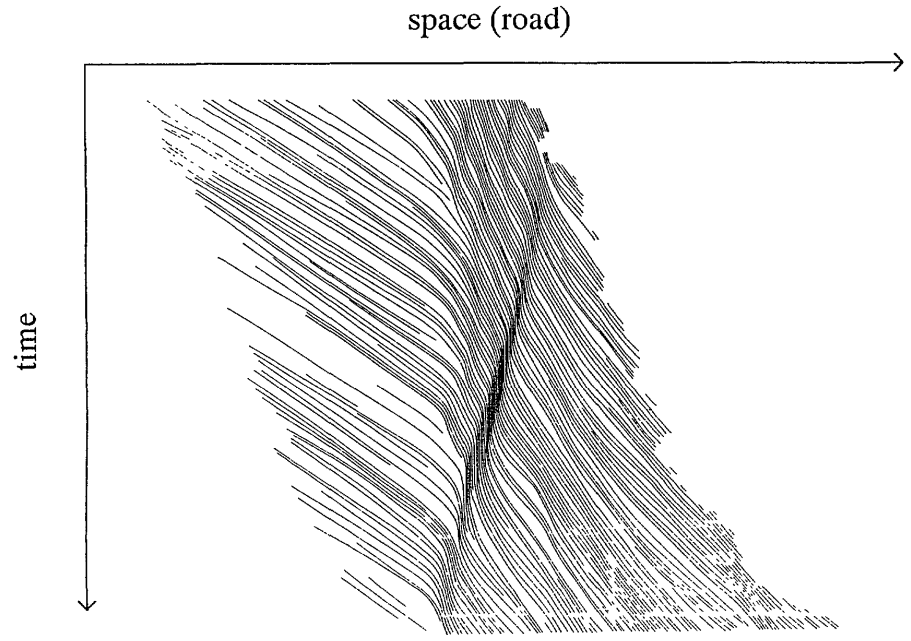
\includegraphics[width=0.8\linewidth]{images/nasch_space_time_diagram.png}
    \caption{Space-time-lines for cars from Aerial Photography \cite{NASCH1992}.}
    \label{fig:nasch_space_time_diagram}
\end{figure}

The model demonstrates that the traffic flow initially increases with the vehicle density, reaches a maximum, and then decreases as density increases, see figure \ref{fig:nasch_flow_density_diagram}. However, the exact position of the maximum can vary depending on the system size, making it difficult to determine the transition point\cite{NASCH1992}.

\begin{figure}
	\centering
    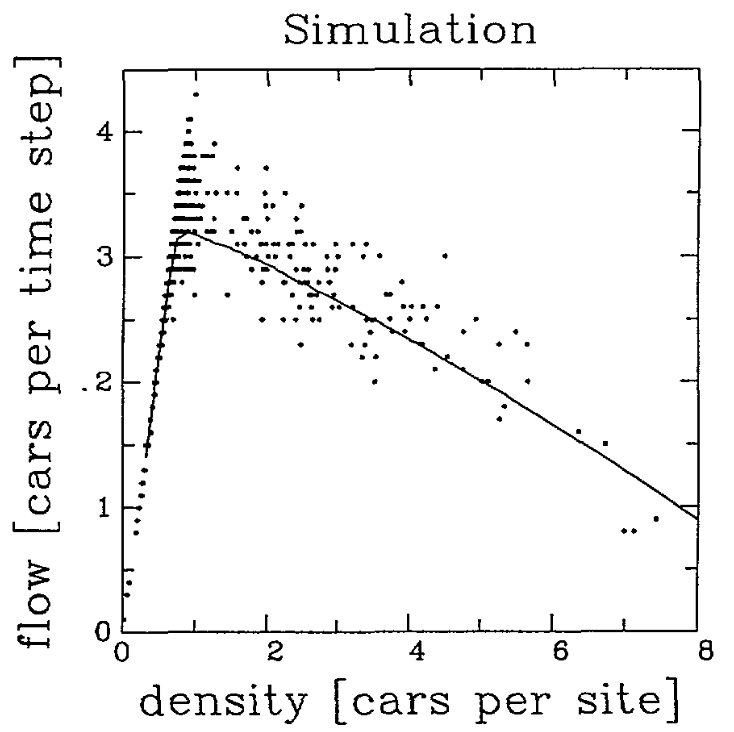
\includegraphics[width=0.8\linewidth]{images/nasch_flow_density_diagram.png}
    \caption{The flow-density diagram for the simulation of a one-lane street is shown with dots as the average over 100 steps and a line representing the average of a million time steps. This diagram represents the flow of traffic on the street and how it changes with density\cite{NASCH1992}.}
    \label{fig:nasch_flow_density_diagram}
\end{figure}

According to K. Nagel and M. Schreckenberg, the length and time scales of the model should be calibrated based on realistic traffic data. One such method is to use 7.5 meters, the average space occupied by a car in a traffic jam, as the length of a tile. With an average speed of 120 km/h on a German motorway, this translates to a car moving 4.5 tiles per time step. Thus, a time step in the model should be approximately one second, as following calculation \ref{eq:Nasch_time_step} shows \cite{NASCH1992}:
    \begin{align}
        7.5[\frac{m}{site}] * 4.5 [\frac{sites}{timestep}] / (120/3.6)[\frac{sec}{m}]\approx 1[\frac{sec}{timestep}]
        \label{eq:Nasch_time_step}
    \end{align}
These assumptions help to create a simple and realistic simulation of traffic flow on freeways.  K. Nagel and M. Schreckenberg's model results were then compared with aerial photographs, which supported their findings.

\section{Two Lane Traffic Simulations using Cellular Automata}
\label{sec:Two Lane Traffic Simulations using Cellular Automata}
Rickert et al. expanded upon the work of Nagel and Schreckenberg by introducing a two-lane traffic flow model that allows a wider range of vehicles (although the paper only covers cars). With two lanes, differences in speed can be accounted for, unlike the single-lane model, where the average velocity would be limited by the slowest vehicle. The two-lane model proposed by Rickert et al. involves a two-step update process\cite{RICKERT1996534}.: 

\begin{enumerate}
    \item Sideways rules: Vehicles change lanes only by moving sideways, not forward. This sidestep rule is implemented in parallel, with each vehicle making its decision at the start of each step. The lane change decision of a car is based on:
    \begin{enumerate}
        \item The available space in the lane ahead.
        \item The space available in the other lane.
        \item If changing lanes would obstruct another vehicle.
    \end{enumerate}
    \item Single lane update:  Each lane updates its state according to the single update rules described in K. Nagel and M. Schreckenberg's model, see section \ref{sec:A cellular automaton model for freeway traffic}.
\end{enumerate}

Rickert et al. identified the following key parameters for their two-lane traffic flow model:
\begin{itemize}
\item Symmetry: The lane change rules can either be symmetric, applying equally to both lanes, or asymmetric, with cars always attempting to return to the right lane regardless of conditions on the left lane.
\item Stochastic: Deterministic models are considered unrealistic in this context. A lack of randomization combined with parallel updating can lead to synchronized lane changes. The cluster dissolves only until the maximum speed is reached or the cluster is overtaken by other vehicles. This phenomenon of "ping-pong" lane changes is also prevalent in the asymmetric case. 
\item Direction of causality: In the single-lane model, the direction of causality is opposite to the direction of vehicle flow. However, in the two-lane model, vehicles must check the other lane before changing, resulting in causality pointing in the direction of vehicle flow. 
\end{itemize}

Rickert et al. found that the lane change rate was higher in the asymmetric model as expected. They also demonstrated that reducing the lane change probability from 1 to 1/2 significantly reduced the number of "ping-pong" lane changes, suggesting that the phenomenon was caused by tailgating.
For consistency with real-world behavior, the vehicle's lookahead should be set to $v+1$, not just $v$. This adjustment is minor for vehicles in motion, but crucial for those in traffic jams, which would otherwise fail to consider lane changes. Reducing the look-back behavior to zero should also be avoided, as it leads to abrupt stops for obstructed vehicles and disrupts the smooth flow of traffic.

\section{Traffic dynamics of carnival processions}
\label{sec:Traffic dynamics of carnival processions}
The paper by Polichronidis \cite{Polichronidis_2018} uses a cellular automata model to examine the dynamics of the Cologne Rose Monday Parade. This procession can be considered as a long, one-lane traffic jam, and the model captures its spatial contraction. The parade moves at a constant speed and any unexpected brakes at the front result in accumulative brakes at the back, leading to a higher average velocity for the rear participants. The spread of the disruption is depicted through a time-distance diagram for each vehicle see figure \ref{fig:polichronidis_time_distance}. This observation suggests that some event occurred around 1:30 pm and 3:30 pm that caused a disturbance or delay in the parade group, which then propagated backwards through the group. This could be due to a variety of factors, such as a roadblock, an accident, a technical problem with one of the vehicles, or some other unexpected event.
\begin{figure}
	\centering
    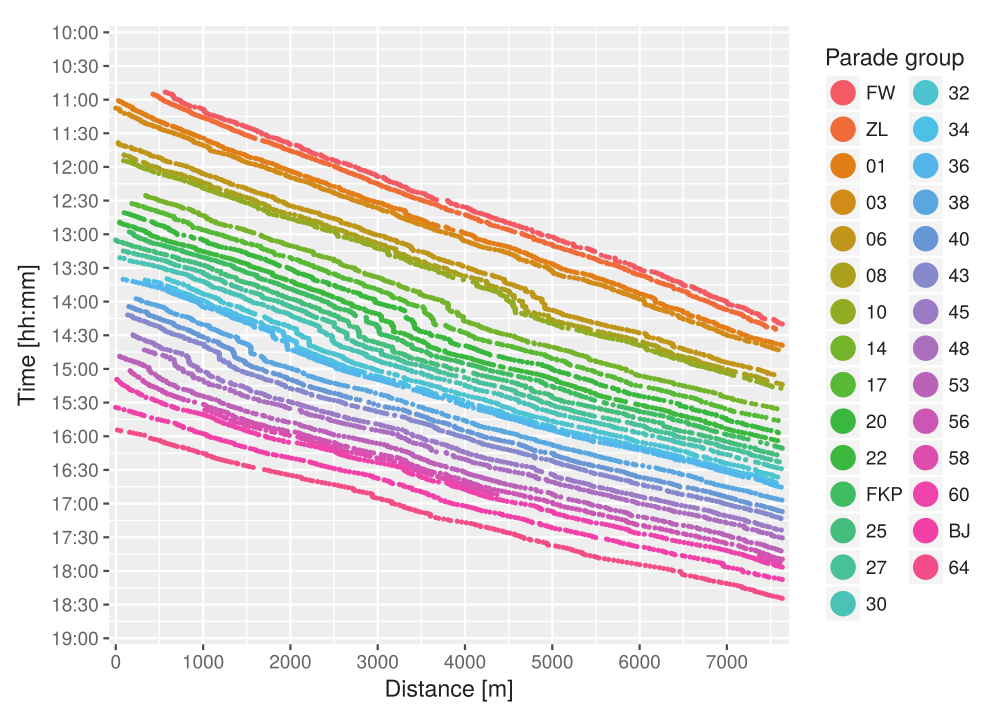
\includegraphics[width=0.8\linewidth]{images/polichronidis_time_distance.png}
    \caption{Time-distance diagram of the 2014 Rose Monday parade \cite{Polichronidis_2018}.}
    \label{fig:polichronidis_time_distance}
\end{figure}
Although traffic jams typically cause delays, this is not the case for the parade, where even spontaneous local congestion do not result in an overall delay. This is partly due to the limiting factor of the front vehicle increasing its escape speed from the parade queue and partly due to the spatial contraction of the parade. The paper's findings are supported by GPS data summarized in figure \ref{fig:polichronidis_velo_distribution}.
\begin{figure}
	\centering
    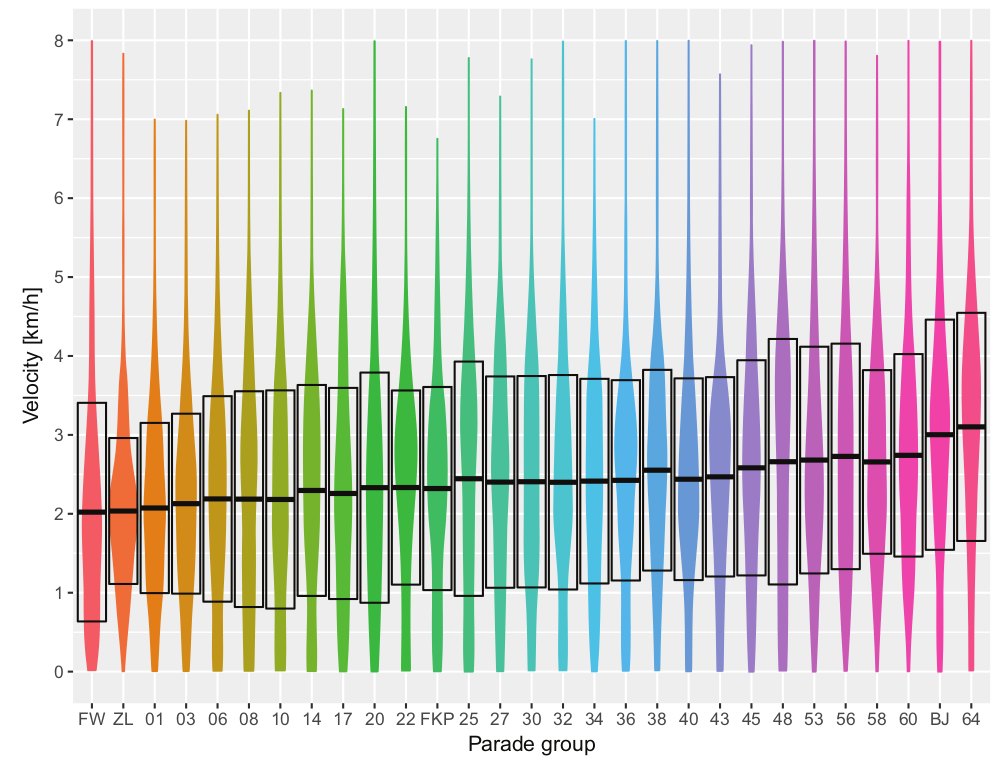
\includegraphics[width=0.8\linewidth]{images/polichronidis_velo_distribution.png}
    \caption{Velocity distributions of the participants in the 2014 Rose Monday parade. Boxes represent the standard deviation. The box located at the farthest right side symbolizes the end segment of the parade \cite{Polichronidis_2018}.}
    \label{fig:polichronidis_velo_distribution}
\end{figure}










% This command is only for filling the bibliography in this example and must not be used in your thesis.
\nocite{*}